\section{Architecture High Level Diagrams}

%\begin{center}
%	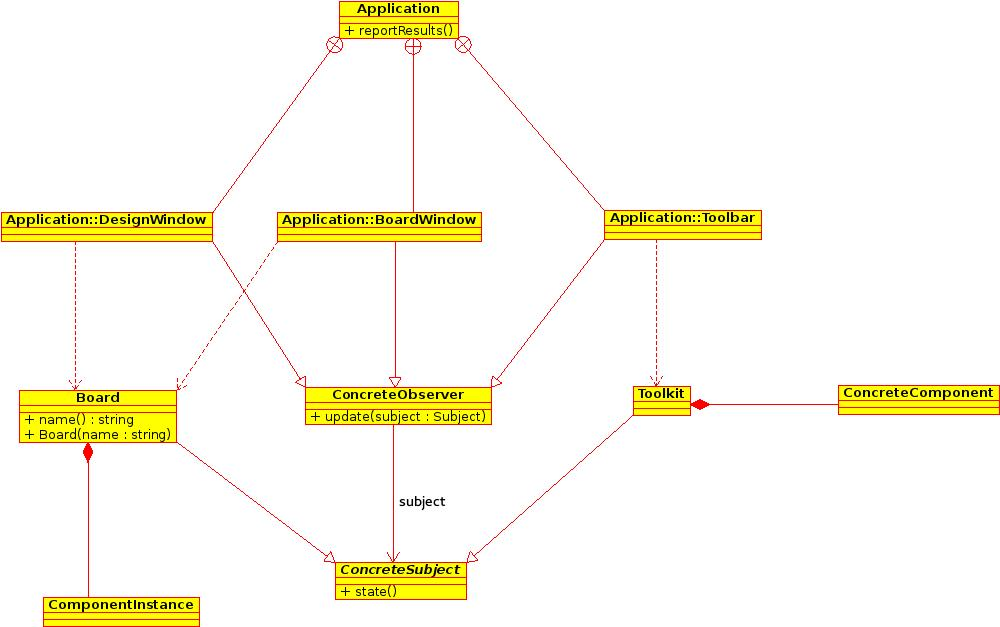
\includegraphics[width=.9\linewidth]{UI_ClassDiagramMain.jpeg}
%	\captionof{figure}{User Interface high level class diagram}
%	\label{fig:ui_class_diagram}
%\end{center}

\todo[inline]{To do}

\section{Plugin requirements}

\begin{description}
	\item[01] Plugin must receive a data model representing the
	network as containing only the primitives intel designed.

	\item[02] Plugin must be able to walk the data model by DFS or BFS 
	define its own visit activities.

	\item[03] Plugin must be able to add data to the data model without
	modifying the data model.
	
	\item[04] Plugin must be able to send results back to the caller
	or to a following plugin.
	
	\item[99] \todo[inline]{To be finished}
\end{description}

\section{Plugin construction}

Any verification tool must override the \w{ConcreteVerificationTool} 
and register with the application in order to have the option
of being executed on request. 



\begin{center}
	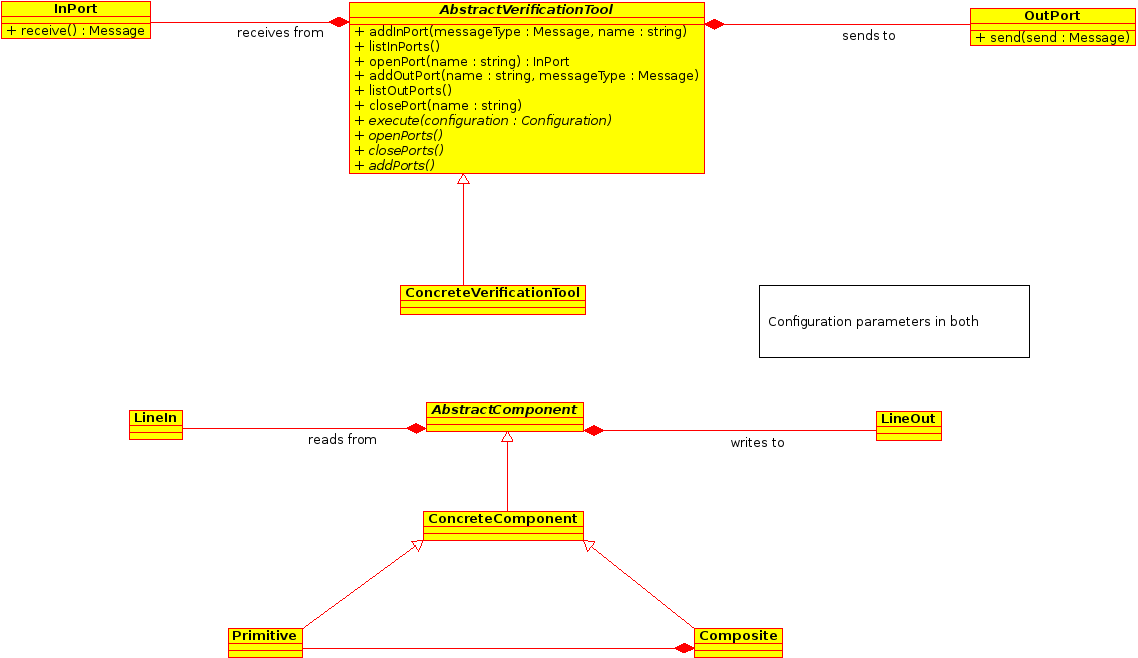
\includegraphics[width=.9\linewidth]{PluginClassDiagram}
	\captionof{figure}{The plugin to build verification tools.}
	\label{fig:plugin-class-diagram}
\end{center}

